\documentclass{article}
\usepackage[utf8]{inputenc}
\usepackage[english]{babel}
\usepackage{geometry}
\geometry{a4paper, margin=1in}
\usepackage{titlesec}
\usepackage{hyperref}
\usepackage{amsmath}
\usepackage{amssymb}
\usepackage{amsthm}
\usepackage{xcolor}
\usepackage{tikz}
\usetikzlibrary{arrows.meta, positioning, calc}

\definecolor{lightblue}{RGB}{220,240,250}
\definecolor{darkblue}{RGB}{20,60,120}
\definecolor{lightgrey}{RGB}{230,230,230}

\titleformat{\section}
  {\normalfont\Large\bfseries}{\thesection.}{1em}{}
\titleformat{\subsection}
  {\normalfont\large\bfseries}{\thesubsection.}{1em}{}

% --- Title Page Setup ---
\title{Linear Algebra Vocabulary Reference}
\author{Your Name / Course Name}
\date{\today}

\begin{document}

% --- Title Page ---
\begin{titlepage}
    \centering
    \vspace*{2cm}
    {\Huge\bfseries Linear Algebra Vocabulary\par}
    \vspace{1cm}
    {\Large A Comprehensive Glossary\par}
    \vfill
    {\Large Haadi Majeed / EN.625.252.81 Fall 2025\par}
    \vfill
    {\large \today \par}
    \vspace{2cm}
\end{titlepage}

% --- Table of Contents ---
\newpage
\tableofcontents
\newpage % Start the content on a new page

% --- Vocabulary Sections ---

\section{Module 2}
\subsection{Parallelogram Rule for Addition}

    \vspace{1cm}
    \begin{center}
    \colorbox{lightblue}{\parbox{0.9\textwidth}{
    \textbf{\color{cyan!80!black} Parallelogram Rule for Addition, Lay 1.3}

    If \(\mathbf{u}\) and \(\mathbf{v}\) in \(\mathbb{R}^2\) are represented as points in the plane, then \(\mathbf{u} + \mathbf{v}\) corresponds to the fourth vertex of the parallelogram whose other vertices are \(\mathbf{u}\), \(\mathbf{0}\), and \(\mathbf{v}\). See Figure 3.
    }}
    \end{center}

    \vspace{1cm}

    \begin{center}
    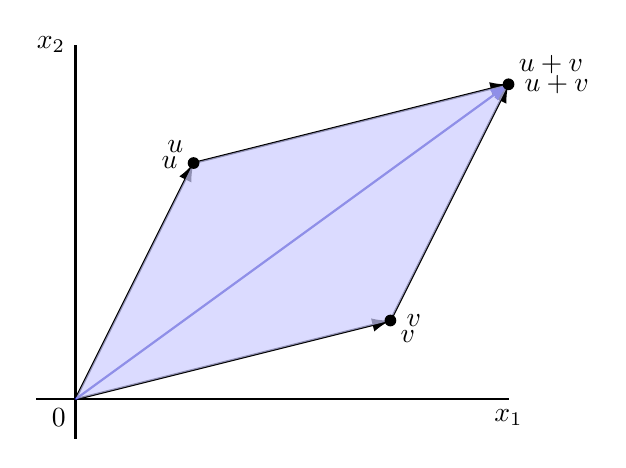
\begin{tikzpicture}[
        >=Latex,
        vector/.style={thick, ->, black},
        result_vector/.style={thick, ->, blue!70!black},
        axis/.style={thick, black},
        point/.style={circle, fill, inner sep=1.5pt}
        ]
        % Axes
        \draw[axis] (-0.5,0) -- (5.5,0) node[below] {\(x_1\)};
        \draw[axis] (0,-0.5) -- (0,4.5) node[left] {\(x_2\)};

        % Origin
        \node[below left] at (0,0) {\(0\)};

        % Vectors u and v
        \coordinate (O) at (0,0);
        \coordinate (U) at (1.5, 3);
        \coordinate (V) at (4, 1);

        \draw[vector] (O) -- (U) node[above left, font=\bfseries] {\(u\)};
        \draw[vector] (O) -- (V) node[below right, font=\bfseries] {\(v\)};

        % Parallelogram lines (dashed)
        \draw[vector] (U) -- ($ (U) + (V) $) node[above right, font=\bfseries] {\(u+v\)};
        \draw[vector] (V) -- ($ (U) + (V) $);

        % Resultant vector u+v
        \draw[result_vector] (O) -- ($ (U) + (V) $);

        % Shaded parallelogram region
        \fill[blue!20, opacity=0.7] (O) -- (U) -- ($ (U) + (V) $) -- (V) -- cycle;

        % Points for the vectors
        \node[point, label=left:\(u\)] at (U) {};
        \node[point, label=right:\(v\)] at (V) {};
        \node[point, label=right:\(u+v\)] at ($ (U) + (V) $) {};


    \end{tikzpicture}
    \end{center}
\subsection{Algebraic Properties}
    \vspace{1cm}
    \begin{center}
    \colorbox{lightblue}{\parbox{0.9\textwidth}{
    \textbf{\color{cyan!80!black}Algebraic Properties of \(\mathbb{R}^n\)}

    For all \(\mathbf{u}\), \(\mathbf{v}\), \(\mathbf{w}\) in \(\mathbb{R}^n\) and all scalars \(c\) and \(d\):
    \begin{enumerate}
        \item \(\mathbf{u} + \mathbf{v} = \mathbf{v} + \mathbf{u}\)
        \item \((\mathbf{u} + \mathbf{v}) + \mathbf{w} = \mathbf{u} + (\mathbf{v} + \mathbf{w})\)
        \item \(\mathbf{u} + \mathbf{0} = \mathbf{0} + \mathbf{u} = \mathbf{u}\)
        \item \(\mathbf{u} + (-\mathbf{u}) = -\mathbf{u} + \mathbf{u} = \mathbf{0}\), \\
            where \(-\mathbf{u}\) denotes \((-1)\mathbf{u}\)
        \item \(c(\mathbf{u} + \mathbf{v}) = c\mathbf{u} + c\mathbf{v}\)
        \item \((c + d)\mathbf{u} = c\mathbf{u} + d\mathbf{u}\)
        \item \(c(d\mathbf{u}) = (cd)\mathbf{u}\)
        \item \(1\mathbf{u} = \mathbf{u}\)
    \end{enumerate}
    }}
    \end{center}

\subsection{Linear Combination and Span}
    \vspace{1cm}
    \colorbox{darkblue}{\parbox{\textwidth}{\centering \color{white}
    \Large\bfseries A linear combination, definition, Lay, 1.3
    }}
    \vspace{0.5cm}

    Let \(\mathbf{v}_1, \mathbf{v}_2, \ldots, \mathbf{v}_p\) be vectors in \(\mathbb{R}^n\).
    \vspace{0.5cm}

    \textcolor{red}{A linear combination} of \(\mathbf{v}_1, \mathbf{v}_2, \ldots, \mathbf{v}_p\) is a vector
    \[
    c_1\mathbf{v}_1 + c_2\mathbf{v}_2 + \dots + c_p\mathbf{v}_p, \quad c_1, c_2, \ldots, c_n \in \mathbb{R}
    \]
    \vspace{0.5cm}

    \textcolor{red}{The span} of \(\mathbf{v}_1, \mathbf{v}_2, \ldots, \mathbf{v}_p\) is the set of all linear combinations
    \[
    \{ c_1\mathbf{v}_1 + c_2\mathbf{v}_2 + \dots + c_p\mathbf{v}_p, \quad c_1, c_2, \ldots, c_n \in \mathbb{R} \}
    \]

\subsection{Properties of Matrix-Vector Product}
    \vspace{1cm}
    \begin{center}
    \colorbox{lightblue}{\parbox{0.9\textwidth}{
    If \(A\) is an \(m \times n\) matrix, \(\mathbf{u}\) and \(\mathbf{v}\) are vectors in \(\mathbb{R}^n\), and \(c\) is a scalar, then:
    \begin{enumerate}
        \item[a.] \(A(\mathbf{u} + \mathbf{v}) = A\mathbf{u} + A\mathbf{v}\);
        \item[b.] \(A(c\mathbf{u}) = c(A\mathbf{u})\).
    \end{enumerate}
    }}
    \end{center}

\end{document}
